% Since \input doesn't like preambles, only uncomment next line if you're editing this TeX, don't forget the \end{document}! 
%\documentclass{article}\usepackage[utf8]{inputenc} % allows for non-ASCII characters
\usepackage[x11names]{xcolor}    % Color extensions
\usepackage[margin=1in]{geometry} % Formatting on page
\usepackage{array} % big arrays
\usepackage{amsmath} % Math symbols
\usepackage{amsthm}   
\usepackage{amssymb}
\usepackage[backend=bibtex]{biblatex} % bibliography
\usepackage{bm} % bold for greek letters
\usepackage{cancel}
\usepackage[format=hang]{caption}
\usepackage{enumitem} % Enumerating things
\usepackage{esint} % better double and triple Integrals
\usepackage{etoc}
\usepackage{fancyhdr} % Headers
    \pagestyle{fancy}
\usepackage{float}
\usepackage{gensymb}
\usepackage{physics} % easier commands for physics things
\usepackage{relsize}  % allows for larger/smaller math 
\usepackage{textcomp} % Gets rid of perthousand error
\usepackage{upquote}  % fixes quotes in verbatim environment
\usepackage{verbatim} % Allows for comment environment
\usepackage{tikz} % pictures
	\usetikzlibrary{calc}
	\usetikzlibrary{decorations.markings}
	\usetikzlibrary{3d}
	\usetikzlibrary{intersections}
\usepackage{pgfplots} % plots and graphics
	\pgfplotsset{compat=newest} % or use compat=1.6
	\usepgfplotslibrary{fillbetween}
\usepackage{graphicx} % plots and graphics
\usepackage{wrapfig}
\usepackage{xparse} % Better commands
\usepackage[hidelinks]{hyperref}% References--THIS GOES LAST

% Packages that this breaks without: amsmath, gensymb, physics, hyperref, xcolor, xparse, and possibly others
\numberwithin{equation}{section} % amsmath command that renews equation counter in each section\
\def\ints{\int_\mathcal{S}} % Surface integral
\def\intv{\int_\mathcal{V}} % Volume integral with V subscript
\def\intall{\int_{-\infty}^{\infty}} % Integral over all space
\def\iintall{\iint_{\rm All Space}} % Integral over all space
\def\iiintall{\iiint_{\rm All Space}} % Integral over all space
\def\ik{4\pi\epsilon_0} % Inverse k for EM
\def\lap{\mathcal{L}}
\def\answerline{ % double horizontal line placed 0.5 cm below text, space between lines is 0.07 cm, then 0.75 cm of space 
	\vspace{0.5 cm}
	\hrule
	\vspace{0.07 cm}
	\hrule
	\vspace{0.75 cm}\noindent} % don't indent text after the line
\NewDocumentCommand\length{O{3pt}}{\setlength\jot{#1}} % for align vertical spacing, there's probably a better way to do this locally
\NewDocumentCommand\ft{s O{n} O{L}}{ % I dont want to write \sin(stuff) \cos(stuff) every time in fourier transforms (ft)
    \IfBooleanTF{#1}{
        \sin(\frac{#2 \pi}{#3}x)
    }{
        \cos(\frac{#2 \pi}{#3}x)
    }
}

\NewDocumentCommand\dl{s}{\IfBooleanTF{#1}{}{\cdot} d\mathbf{l}} % quicker curve integral dl, if no star, it also makes the dot 
\NewDocumentCommand\da{s}{\IfBooleanTF{#1}{}{\cdot} d\mathbf{a}} % quicker surface integral da, if no star, it also makes the dot 
\NewDocumentCommand\oo{O{1} m} {\frac{#1}{#2}}   % reciprocal- 'one over', option to make it a regular fraction because oo is still quicker to type.
\NewDocumentCommand\thetitle{m O{}}{ \title{ \hypertarget{top}{\textbf{#1}} \\ \large {#2} } } %Bold title that is a hypertarget, optional bolded subtitle that's scaled properly 

\NewDocumentCommand \e {s m}{ % basis vector command
	\IfBooleanTF{#1} % \e{x} for x hat notation, \e*{x} for e_x notation
	{\mathbf{\hat{e}_{#2}}}
	{\bm{\hat{#2}}}} % from package bm, more powerful than \mathbf} 
\NewDocumentCommand \parametric {m}{ %command for getting boundary conditions with a "{" on the left
    \left\{ 
	\begin{gathered}
		\begin{matrix}
			#1
    		\end{matrix}
	\end{gathered}
	 \right.}
\NewDocumentCommand \der {s O{} m g}{ % custom derivative command
     \IfBooleanTF{#1} % if \der*, #1 is true, euler notation used, if \der , #1 is false, d/dx is used 
    {\IfNoValueTF{#4}  % g returns -NoValue- if no argument (read below)
        {\mathrm{D}_{#3}^{#2}}  % g is included so \der{x} and \der{f}{x} both have x in the denominator
        {\mathrm{D}_{#4}^{#2}#3}
            }
    {\IfNoValueTF{#4}
        {\frac{\mathrm{d}^{#2}}{\mathrm{d} #3^{#2}}}
        {\frac{\mathrm{d}^{#2} #3}{\mathrm{d} #4^{#2}}}
	}}    
\NewDocumentCommand \pder {s O{} m g}{ % custom partial derivative command, allows for euler notation if starred
     \IfBooleanTF{#1}
        {\IfNoValueTF{#4}
            {\partial_{#3}^{#2}}
            {\partial_{#4}^{#2}#3}
                }
        {\IfNoValueTF{#4}
            {\frac{\partial^{#2}}{\partial #3^{#2}}}
            {\frac{\partial^{#2} #3}{\partial #4^{#2}}}
                }} 
                
\NewDocumentCommand \header {m m m}{
	\fancyhead[L]{#1} 
	\fancyhead[C]{\hyperlink{top}{ \textbf{#2} }}
	\fancyhead[R]{#3}
	\fancyfoot[C]{--\thepage--}
	\pagestyle{fancy}
	\setlength\headheight{17pt}}
    
\NewDocumentCommand{\coloredanswer}{O{LavenderBlush2} m}{ % makes coloredbox with pretty color
	\mathchoice
	{\colorbox{#1}{$\displaystyle #2$}}
	{\colorbox{#1}{$\textstyle #2$}}
	{}
	{}}

\newcounter{probcount} % new counter for problem numbers, starts at 0 by default
\NewDocumentEnvironment{ problem } {O{} +b} %Problem environment for homework, autocounts numbers, behaves like a section and can get listed (and hyperlinked) in the toc. 
	{\addtocounter{probcount}{1} % increase counter at the beginning of every problem
	 \phantomsection % invisible page marker for hyperref
	 \addcontentsline{toc}{subsection}{Problem \theprobcount. {\it#1}} % add "Problem \theprobcount. \textit{#1}" to table of contents (toc) as if it were a subsection
	 \begin{trivlist} % begin unmarked ("trivial") list
	 \item {\bf Problem \theprobcount.} {\it#1} % print Problem with the counter and optional text 
	 \item #2  % +b is for inputs that are long
	 \end{trivlist} % end list
	}{} % don't do anything then "problem" environment ends, irrelevant because trivlist is already ended
	
\def\UM{\colorbox{blue}{\textcolor{Gold1}{\textbf{University of Michigan}}}} % School Pride
\def\EC{\href{https://github.com/CarpenterEvan/PhysicsReview}{\(\mathbb{E}\textsc{van}~\mathbb{C}\textsc{arpenter}\)}}
\endinput\begin{document}
\section{Curvilinear Coordinates}
\subsection{Spherical Coordinates}
    In this system of coordinates, the following describe the space's basis set:
    %\tikzsetnextfilename{spherical}
    \tikzfading[name=ball, outer color=transparent!50, inner color=transparent!100]
    \begin{figure}[H]
        \begin{tikzpicture}
            \draw [dotted] (2.3,0,2)--(2.3,2.3,2)--(0,2.3,0); % projection of r onto z and x axis
            \draw [orange!30, fill=orange!30] (0,0,0)--(0.75,0.75,0) arc [start angle=45, end angle=90,radius=10 mm] node at (0.25,0.7) [black] {$\theta$}; % Theta arc
            \begin{scope}[canvas is xz plane at y=0]
                \draw [dotted] (0,0)--(2.3,2);
                \fill [blue!20] (0,0)--(1.2,1) arc [start angle=45, end angle=120,radius=10 mm] node at (0.35,0.65) [black] {$\phi$};
            \end{scope}


            %\fill [path fading=ball, color=black] (0.07,0) circle (2.5);
            \draw [ultra thick, -latex] (0,0,0)--(3,0,0) node [anchor=north west] {\textbf{y}};
            \draw [ultra thick, -latex] (0,0,0)--(0,3,0) node [anchor=south]      {\textbf{z}};
            \draw [ultra thick, -latex] (0,0,0)--(0,0,3) node [anchor=north west] {\textbf{x}};


            \draw [ultra thick, blue!20, -latex] (2.3,2.3,2)--(3,2,0.7) node [anchor=west, color=black] {$\e{\phi}$}; 
            \draw [ultra thick, orange!30, -latex] (2.3,2.3,2)--(3,1.6,2.25) node [anchor= north, color=black] {$\e{\theta}$}; 
            \draw [ultra thick, blue, -latex] (2.3,2.3,2)--(3,3,2) node [anchor=south east, color=black] {$\e{r}$}; 
            \draw [ultra thick, red, -latex] (0,0,0)--(2.3,2.3,2) node at (1,0.5) {\textbf{r}};


            \node (description text) at (6,2,0) {Distance from the origin: r};
            \node at (description text.south) [xshift=29.5, yshift=-5] {Polar angle: $\theta$};
            \node at (description text.south) [xshift=19, yshift=-16] {Azimuthal angle: $\phi$};
        \end{tikzpicture}
    \end{figure}
    Important relationships:
    \begin{align*}
        \begin{bmatrix}
        \e{r}\\
        \e{\theta}\\
        \e{\phi}
        \end{bmatrix}
        &=
        \begin{bmatrix}
        \sin(\theta)\cos(\phi)&\sin(\theta)\sin(\phi)&\cos(\theta)\\
        \cos(\theta)\cos(\phi)&\cos(\theta)\sin(\phi)&-\sin(\theta)\\
        -\sin(\phi)&\cos(\phi)&0
        \end{bmatrix}
        \begin{bmatrix}
        \e{x}\\
        \e{y}\\
        \e{z}
        \end{bmatrix}
    \end{align*}
    \begin{center}
    Matrix is orthogonal, transpose to find $\e{x}$ in terms of $\e{r}$
    \end{center}
    \vspace{0.5 cm}
    Position, velocity, and acceleration:
    \begin{align*}
        \vb{r}(t)&=
        \begin{bmatrix}
        r
        \\
        0
        \\
        0
        \end{bmatrix}
        \cdot
        \begin{bmatrix}
        \e{r}
        \\
        \e{\theta}
        \\
        \e{\phi}
        \end{bmatrix}
        \\
        \vb{v}(t)&=
        \begin{bmatrix}
        \dot{r}
        \\
        r\dot{\theta}
        \\
        r\dot{\phi}\sin(\theta)
        \end{bmatrix}
        \cdot
        \begin{bmatrix}
        \e{r}
        \\
        \e{\theta}
        \\
        \e{\phi}
        \end{bmatrix}
        \\
        \vb{a}(t)&=
        \begin{bmatrix}
        \Ddot{r}-r\dot{\theta}^2-r\dot{\phi}^2\sin^2(\theta)
        \\
        r\Ddot{\theta}+2\dot{r}\dot{\theta}-r\dot{\phi}^2\sin(\theta)\cos(\theta)
        \\
        2r\dot{\theta}\dot{\phi}\cos(\theta)+2\dot{r}\dot{\phi}\sin(\theta)+r\Ddot{\phi}\sin(\theta)
        \end{bmatrix}
        \cdot
        \begin{bmatrix}
        \e{r}\\
        \e{\theta}\\
        \e{\phi}
        \end{bmatrix}
    \end{align*}
    \newpage\noindent
    Infinitesimal Displacement:
    \[\dl* = dr\ \e{r} + r d\theta\ \e{\theta} + r \sin(\theta) d\phi\ \e{\phi} \]
    Infinitesimal Areas:
    \begin{align*}
        \begin{tabular}{|c|c|}
            \hline
            Held Constant & $\da*$ \\ 
            \hline
            r & $r^2 \sin(\theta) d\theta d\phi\ \e{r}$\\ 
            \hline
            $\theta$ & $r \sin(\theta) dr d\phi\ \e{\theta}$ \\ 
            \hline
            $\phi$ & $r dr d\theta\ \e{\phi}$\\
            \hline
        \end{tabular}
    \end{align*}
    Infinitesimal volume: \[dV = r^2\sin(\theta) dr d\theta d\phi\]
    \subsubsection*{Spherical Vector Derivatives:}
        {\setlength\jot{1cm}
        \renewcommand{\arraystretch}{1.5}
        \begin{align*}
            \text{Gradient:}&&
            &\nabla f = 
            \qty[
            \begin{matrix}
                \pder*{f}{r}
                \\
                \frac{1}{r} \pder*{f}{\theta}
                \\
                \frac{1}{r \sin(\theta)}\pder*{f}{\phi}
            \end{matrix}
            ]\cdot\qty[
            \begin{matrix}
                \e{r}\\\e{\theta}\\\e{\phi}
            \end{matrix}
            ]
            \\
            \text{Divergence:}&&
            \div \vb{A} &= \oo{r^2}\pder*{r}\qty(r^2A_r) 
            + \oo{r \sin(\theta)} \pder*{\theta} \qty(\sin(\theta)A_\theta) 
            + \oo{r \sin(\theta)} \pder*{A_\phi}{\phi}
            \\
            \text{Curl:}&&
            &\curl \vb{A} = 
            \qty[
               \begin{matrix}
                    \oo{r\sin(\theta)}\qty[\pder*{\theta}\qty(A_\phi\sin(\theta))-\pder*{A_\theta}{\phi}]
                    \\
                    \oo{r\sin(\theta)}\pder*{A_r}{\phi}-\oo{r}\pder*{r}\qty(r A_{\phi})
                    \\
                    \frac{1}{r}\qty(\pder*{r}\qty(rA_{\theta}) - \pder*{\theta}A_r)
                \end{matrix}
            ]\cdot\qty[
            \begin{matrix}
                \e{r} \\\e{\theta} \\\e{\phi}
            \end{matrix}]
            \\
            \text{Scalar Laplacian:}&&
            \nabla^2 f 
            &= \frac{1}{r^2} \pder{r}\qty(r^2 \pder{f}{r}) + \oo{r^2 \sin(\theta)} \pder{\theta} \qty(\sin(\theta)\pder{f}{\theta}) +\frac{1}{r^2 \sin^2(\theta)} \pder[2]{f}{\phi}
        \end{align*}}


\newpage
\subsection{Cylindrical Coordinates}
    In this system, the following describe the space's basis set:
    %\tikzsetnextfilename{cylindrical}
    \begin{figure}[H]
        \begin{tikzpicture}  
            \draw [dotted] (0,0,0)--(2.3,0,2)--(2.3,2.3,2)--(0,2.3,0);
            \begin{scope}[canvas is xz plane at y=0]
                \fill [blue!20] (0,0)--(1.2,1) arc [start angle=45, end angle=120,radius=10 mm] node at (0.35,0.65) [black] {$\phi$};
            \end{scope}
            \draw [ultra thick, -latex] (0,0,0)--(3,0,0) node [anchor=north west] {\textbf{y}};
            \draw [ultra thick, -latex] (0,0,0)--(0,3,0) node [anchor=south] {\textbf{z}};
            \draw [ultra thick, -latex] (0,0,0)--(0,0,3) node [anchor=north west] {\textbf{x}};


            \draw [ultra thick, blue!20, -latex] (2.3,2.3,2)--(2.7,2,0.7) node [anchor=west, color=black] {$\e{\phi}$}; 
            \draw [ultra thick, brown, -latex] (2.3,2.3,2)--(3.5,2.3,3.043) node [anchor=north west, color=black] {$\e{s}$}; 
            \draw [ultra thick, blue, -latex] (2.3,2.3,2)--(2.3,3,2) node [anchor=south east, color=black] {$\e{\textbf{z}}$}; 


            \draw [ultra thick, red, -latex] (0,0,0)--(2.3,2.3,2) node at (1,0.5) {\textbf{r}};
            \draw [ultra thick, -latex, brown] (0,0,0)--(2.3,0,2) node [anchor=west] {\textbf{s}};
            \draw [ultra thick, -latex, blue] (0,0,0)--(0,2.3,0) node [anchor=east] {\textbf{z}};


            \node (description text) at (6,2,0) {Distance from the z-axis: s};
            \node at (description text.south) [xshift=29.5, yshift=-5] {Azimuthal angle: $\phi$};
            \node at (description text.south) [xshift=19, yshift=-16] {Distance on z-axis: z};
        \end{tikzpicture}
    \end{figure}
    Important relationships:
    \begin{align*}
        \begin{bmatrix}
        \e{s}\\
        \e{\phi}\\
        \e{z}
        \end{bmatrix}
        &=
        \begin{bmatrix}
        \cos(\phi)&\sin(\phi)&0\\
        -\sin(\phi)&\cos(\phi)&0\\
        0&0&1
        \end{bmatrix}
        \begin{bmatrix}
        \e{x}\\
        \e{y}\\
        \e{z}
        \end{bmatrix}
    \end{align*}
    \begin{center}
    Matrix is orthogonal, transpose to find $\e{x}$ in terms of $\e{s}$
    \vspace{0.5 cm}
    \end{center}
    Position, velocity, and acceleration:
    \begin{align*}
        \vb{r}(t)&=
        \begin{bmatrix}
            s
            \\
            0
            \\
            z
        \end{bmatrix}
        \cdot
        \begin{bmatrix}
            \e{s}
            \\
            \e{\phi}
            \\
            \e{z}
        \end{bmatrix}
        \\
        \vb{v}(t)&=
        \begin{bmatrix}
            \dot{s}
            \\
            s\dot{\phi}
            \\
            \dot{z}
        \end{bmatrix}
        \cdot
        \begin{bmatrix}
            \e{s}
            \\
            \e{\phi}
            \\
            \e{z}
        \end{bmatrix}
        \\
        \vb{a}(t)&=
        \begin{bmatrix}
            \Ddot{s}-r\dot{\phi}^2
            \\
            s\Ddot{\phi}+2\dot{s}\dot{\phi}
            \\
            \Ddot{z}
        \end{bmatrix}
        \cdot
        \begin{bmatrix}
            \e{s}
            \\
            \e{\phi}
            \\
            \e{z}
        \end{bmatrix}
    \end{align*}
    \newpage\noindent
    Infinitesimal Length:
        \[\dl*= ds\ \e{s}+sd\phi\ \e{\phi}+dz\ \e{z}\]
    Infinitesimal Areas:
        \begin{center}
        \begin{tabular}{|c|c|}
            \hline
            Held Constant & $\da*$ \\ 
            \hline
            s & $sd\phi dz\ \e{s}$ \\ 
            \hline
            $\phi$ & $dsdz\ \e{\phi}$  \\ 
            \hline
            z & $sdsd\phi\ \e{z}$\\
            \hline
        \end{tabular}
        \end{center}
    Infinitesimal Volume: \[dV=sdsd\phi dz\]
    \subsubsection*{Cylindrical Vector Derivatives:}
    {\setlength\jot{0.7cm}
        \renewcommand{\arraystretch}{2.2}
    
        \begin{align*}
        % Gradient         {
        \text{Gradient:}&&%\quad
            \nabla f &= 
                \qty(\pder{f}{s})\e{s}+
                \qty(\oo{s} \pder{f}{\phi})\e{\phi}+
                \qty(\pder{f}{z})\e{z}
            \\
        \text{Divergence:}&&%\quad
            \div\vb{A} &= \oo{s}\pder{s}\qty(s A_s) + \oo{s}\pder{A_\phi}{\phi}  + \pder{A_z}{z}
            \\
        \text{Curl:}&&%\quad
            &\mathlarger{\curl \vb{A} = 
            \qty[
            \begin{matrix}
                \oo{s} \pder{A_z}{\phi} - \pder{A_\phi}{z}
                \\
                \pder{A_s}{z} - \pder{A_z}{s}
                \\
                \oo{s}\pder{s}\qty(s A_\phi) - \oo{s}\pder{A_s}{\phi}
            \end{matrix}
            ]\cdot\qty[
            \begin{matrix}
                \e{s}\\\e{\phi}\\\e{z}
            \end{matrix}
            ]}
            \\
            \text{Scalar Laplacian:}&&%\quad
            \nabla^2 f
            &=\oo{s}\pder{s}\qty(s\pder{f}{s}) 
            + \oo{{s}^2}\pder[2]{f}{\phi} 
            + \pder[2]{f}{z} 
        \end{align*}
    }
%\end{document}